\section{Измерение конденсаторов}
Измерение величины ёмкости конденсаторов сделано, как отдельная задача измерения времени зарядки после всех других 
измерений. Оригинальное программное обеспечение от Markus~F. это делает в цикле программы, которая читает 
соответствующие цифровые входы, пока не произошло отключение, и считает количество циклов. У этого способа есть 
ограничение: разрешение измерения времени ограничено временем, требующимся для одного цикла. Это обычно делается 
во всех шести комбинациях для всех трех испытательных выводов. Новое программное обеспечение использует два разных 
способа получения времени зарядки только в трех комбинациях для трех испытательных выводов.

Положительный вывод конденсатора всегда подключен к испытательному выводу с более высоким номером. Если конденсатор 
измеряется параллельно с диодом, полярность может быть в другом порядке.

\subsection{Разрядка конденсатора}
Вы должны всегда разряжать конденсатор прежде, чем подсоединить его к Тестеру. Тестер дополнительно разряжает 
конденсатор перед любым измерением. Если напряжение ниже~\(1300~mV\), конденсатор будет закорочен выходами порта, 
соединенными со входами порта АЦП (порт~C). Я полагаю, что это допустимо, потому что выход порта имеет встроенный 
резистор около \(20~\Omega\).
Рисунок 149 (page 258) технического описания (страница 258) \cite{ATmega8} показывает падение 
напряжения на выходах до \(2~V\). Конечно, я не могу гарантировать, что никакое повреждение не может произойти. 
Я проверил функцию с конденсаторами большими, чем \(15~mF\) много раз, и я никогда не замечал проблемы. Ток должен 
быть ниже указанного предела \(40~mA\) и быстро уменьшен при разрядке. Конечно, повреждение может произойти, если Вы 
не разрядите конденсатор (высокое напряжение) прежде, чем соедините его с Тестером. 

\subsection{Измерение конденсаторов большой ёмкости }
\label{sec:bigcap}
Одна сторона конденсатора подключена к GND. Другая сторона конденсатора подключена через резистор 
\(680~\Omega\) к VCC на \(10~ms\). Впоследствии этот испытательный вывод будет переключен на ввод (высокий импеданс). 
После этого, \(10~ms\) импульса тока, замеряется напряжение на конденсаторе без тока. Если напряжение не достигло 
минимального значения \(300~mV\), импульс зарядки будет повторен до 499 раз. Если после 127 импульсов не достигнуто 
минимальное напряжение \(75~mV\) (приблизительно \(2~s\)), дальнейшая зарядка будет остановлена, потому что \(300~mV\) 
не смогут быть достигнуты остающимися импульсами зарядки. Рисунок~\ref{fig:bigcap} показывает три фазы измерения 
величины ёмкости конденсатора. Величина ёмкости вычисляется по количеству импульсов зарядки и величине достигнутого 
напряжения заряда из таблицы. Таблица содержит коэффициенты, чтобы получить значение в \(nF\) от времени зарядки и 
достигнутого напряжения с шагом \(25~mV\). Промежуточная величина напряжения будет интерполирована.

\begin{figure}[H]
\centering
 \begin{overpic}[width=.93\textwidth]{../FIG/Bigcap.pdf}
  \color{black}
  \put(25,97){\makebox(0,0)[cb]{Quick Discharge of capacitor}}
  \put(25,61){\makebox(0,0)[cb]{10ms Charge Phase of capacitor}}
  \put(25,26){\makebox(0,0)[cb]{Voltage Measurement Phase of capacitor}}
 \end{overpic}
\caption{Разрядка конденсатора и зарядка импульсом \(10~ms\) до напряжения, не достигающего значения \(300~mV\)}
\label{fig:bigcap}
\end{figure}
В результате низкого напряжения заряда измерение происходит намного быстрее, чем в оригинальной версии программного 
обеспечения, потому что это преимущество работает также при разрядке. Таким способом могут быть измерены большие 
конденсаторы. Кроме того, если диод подключен параллельно конденсатору, то он, в большинстве случаев, не нарушает 
измерение, потому что, для большинства диодов, не может быть достигнуто прямое падение напряжения.
Начиная с версии программного обеспечения 1.12k, используется некоторая особенность для измерения остаточного 
напряжения конденсатора перед измерением его ёмкости. В зависимости от предыдущего теста конденсатора, 
остаточное напряжение может быть как положительным, так и отрицательным. Отрицательные напряжения не может 
быть измерено АЦП. По этой причине, напряжение на отрицательном контакте подтягивается резистором \(690~\Omega\)
примерно до \(132~mV\), как показано на рисунке~\ref{fig:CapResidV}. При разности напряжений, измеренных на обеих 
сторонах конденсатора остаточное напряжение может быть измерено при любой полярности. Напряжение положительного 
тестового контакта остается положительным в любом случае, даже если конденсатор имеет отрицательное остаточное 
напряжение несколько \(mV\).

\begin{figure}[H]
\centering
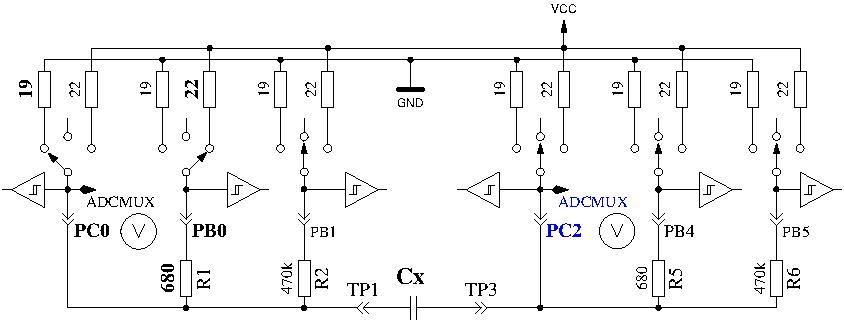
\includegraphics[width=.8\textwidth]{../FIG/Cap_residV.pdf}
\caption{Измерение остаточного напряжения перед зарядом конденсатора}
\label{fig:CapResidV}
\end{figure}

Рисунок~\ref{pic:c229} показывает зарядку и разрядку конденсатора \(229~\mu F\).
Плоская вершина диаграммы от конца зарядки и до начала разрядки вызвана измерением и временем вычисления ATmega. 
Рисунок~\ref{pic:c5mF} показывает такое же измерение конденсатора~\(5~mF\).
Заметьте, что время измерения составило приблизительно \(1,5~s\), включая разрядку.
Последний пример показывает измерение ёмкости конденсатора~\(15~mF\) на рисунке~\ref{pic:c15mF}

\begin{figure}[H]
  \begin{subfigure}[b]{.5\textwidth}
    \centering
    \includegraphics[width=1.\textwidth]{../PNG/charge_229uF.png}
    \caption{\(229~\mu F\) конденсатор}
    \label{pic:c229}
  \end{subfigure}
  ~
  \begin{subfigure}[b]{.5\textwidth}
    \centering
    \includegraphics[width=1.\textwidth]{../PNG/charge_5mF.png}
    \caption{\(5~mF\) конденсатор}
    \label{pic:c5mF}
  \end{subfigure}
  \caption{Зарядка и разрядка конденсатора большой ёмкости для измерения}
\end{figure}

\begin{figure}[H]
  \centering
    \includegraphics[width=.8\textwidth]{../PNG/charge_15mF.png}
  \caption{Зарядка и разрядка конденсатора \(15~mF\) для измерения}
  \label{pic:c15mF}
\end{figure}

После измерения ёмкости конденсатора будет проверен саморазряд ожиданием пропорционально периоду, который 
потребовала зарядка, и снова будет осуществлено считывание напряжения заряда. Взвешенная полная ёмкость будет 
скорректирована из-за этого падения напряжения. Тест с параллельно подключенными конденсатором \(68~\mu F\) и 
резистором \(2,2~k\Omega\) показывает эффективность этого метода. Измеренное  значение ёмкости без 
резистора \(66,5~\mu F\), с параллельным резистором \(2,2~k\Omega\) измеренное значение ёмкости \(66,3~\mu F\).
Для сравнения, результаты, измеренные мультиметром  PeakTech 3315. Без резистора значение ёмкости \(68,2~\mu F\) с 
параллельным резистором \(2,2~k\Omega\) значение ёмкости \(192~\mu F\).


\subsection{Измерение конденсаторов малой ёмкости}
Если первый, \(10~ms\), импульс зарядки перезарядил конденсатор, используется другой алгоритм измерения. У 
микроконтроллера ATmega есть встроенный 16-битный счётчик, который может работать на тактовой частоте 
микроконтроллера (\(1~MHz\) или \(8~MHz\)). У этого счётчика есть также возможность сохранять подсчитанное значение 
внешним сигналом. Этот сигнал может быть выходом компаратора. Компаратор может работать с любым входом АЦП и 
запрещенной зоной опоры. Рисунок~\ref{fig:comparat} показывает упрощенную схему измерения. Итак, я разряжаю 
конденсатор, подключаю компаратор к соответствующему входу, сбрасываю счётчик в 0 и сразу начинаю зарядку 
конденсатора, подсоединённого одной стороной к GND а другой стороной, через резистором \(470~k\Omega\). 
Теперь я проверяю в пределах петли программы переполнение счётчика или сигнал захвата по входу (внешний сигнал). 
Я считаю события переполнения, пока не обнаруживаю входной сигнал захвата. В этом случае я останавливаю счётчик 
и проверяю, не нужно ли подсчитать дополнительное переполнение,  возникшее, пока счётчик не был остановлен входным 
сигналом захвата. 


Входной счётчик захвата и счётчик переполнений совместно определяют полное время, по которому мы можем рассчитать 
фактическую ёмкость. Программное обеспечение использует таблицу с теоретической зависимостью времени зарядки от 
напряжения компаратора. Таблица составлена с шагом \(50~mV\) и будет интерполирована согласно фактическому опорному 
напряжению. Эта таблица будет активна только с опцией WITH\_AUTO\_REF в Makefile. Из полученной величины я вычитаю 
предопределенное, полученное экспериментально, постоянное значение или значение смещение нуля, найденное последней 
самопроверкой с установленной опцией AUTO\_CAL. Смещение нуля может меняться в зависимости от типа печатной платы, 
используемого испытательного оборудования или микроконтроллера. Самопроверка с установленной опцией AUTO\_CAL 
определит смещение нуля автоматически.

 
Я заметил, что стабильность опорного напряжения несколько мала, что Вы можете выбрать опцию REF\_C\_KORR в Makefile. 
После калибровки с опцией AUTO\_CAL, REF\_C\_KORR будет смещением к измеренной разнице напряжений между заряженным 
конденсатором и внутренней опорой. Измеренное опорное напряжение будет тогда добавлено к Вашему значению (в \(mV\)). 
Если опция WITH\_AUTO\_ REF не используется, то применены справочные напряжения для ATmega8, ATmega168 и ATmega328, 
приведенные в технических описаниях ~\cite{ATmega8} и~\cite{ATmega168}. 
Типовое измерение по этому алгоритму показано на рисунке~\ref{pic:c22uF}.
Время измерения для конденсатора \(22~\mu F\) больше \(2,6~s\), потому что для зарядки используется \(470~k\Omega\). 
Но разрядка в этом случае намного быстрее, чем зарядка.

\begin{figure}[H]
\centering
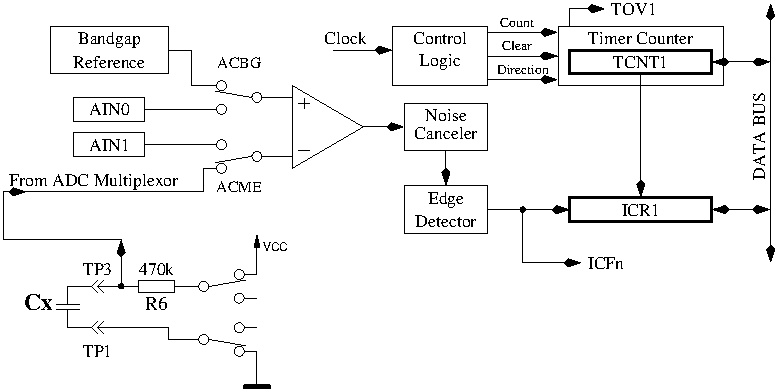
\includegraphics[width=.8\textwidth]{../FIG/Comparat.pdf}
\caption{Измерение малой ёмкости с компаратором}
\label{fig:comparat}
\end{figure}

\begin{figure}[H]
  \centering
    \includegraphics[width=.8\textwidth]{../PNG/charge_22uF.png}
  \caption{Зарядка и разрядка конденсатора \(22~\mu F\) для измерения}
  \label{pic:c22uF}
\end{figure}


В принципе этот алгоритм измерения может также быть проделан с резистором \(680~\Omega\) но, если компаратор работает, 
АЦП не может использоваться, и у меня нет возможности контролировать напряжение заряда, пока компаратор не остановлен. 
Если есть необнаруженный диод, параллельно соединённый с конденсатором, ток зарядки конденсатора может быть поглощен 
диодом (пороговое напряжение), и напряжение запрещенной зоны никогда не будет достигаться. Метод, примененный в 
программном обеспечении для больших конденсаторов в разделе ~\ref{sec:bigcap} не допускает эту концептуальную ошибку.

\subsection{Измерение очень малых значений ёмкости методом выборки}
Радиолюбитель Pieter-Tjerk (PA3FWM) интегрировал возможность измерений очень малых значений ёмкости (\textless~100~pF)
методом выборки.
Период преобразования АЦП на самом деле слишком длительный для непосредственного отбора быстро изменяющегося сигнала.
Но напряжение входного сигнала удерживается заданное время цикла преобразования, во время (\(SH\)) выборки и удержания.
АЦП требуется 13 тактов для полного преобразования, а такты АЦП задаются путем деления частоты процессора на 128 или 64.
Входное напряжение АЦП фиксируется точно 1,5 такта для непрерывных циклов измерений.
Если входной сигнал может быть сгенерирован снова и снова, мы можем сдвинуть время выборки АЦП от предыдущего к 
следующему повторению сигнала, чтобы получить последовательность выборок быстро изменяющегося сигнала.
Обычный цикл АЦП занимает 13x64 = 832 тактов с тактовой частотой \(8~MHz\).
Если мы повторяем входной сигнал с тактовым импульсом 831, то при непрерывном АЦП (режим свободного запуска),
каждый последующий раз напряжение сигнала будет считываться на один такт позже чем предыдущий.
Мы должны убедиться, что с помощью этого метода первая выборка сигнала АЦП будет выполняться в указанное время.
Время следующих измерений АЦП будет сдвинуто на один тактовый импульс процессора позднее при каждом последующем
повторении сигнала.
Если сигнал можно точно повторить, то объединенный сигнал многих периодов будет таким же, как дискретизация и
преобразование непосредственно с помощью АЦП, работающего с тактовым сигналом процессора \(8~MHz\).
Рисунок~\ref{fig:sampling} показывает принцип выборки десятикратно повторяющегося сигнала для получения
десяти выборок (SH0 - SH9).
В действительности относительный временной сдвиг последовательных выборок намного меньше.


\begin{figure}[H]
\centering
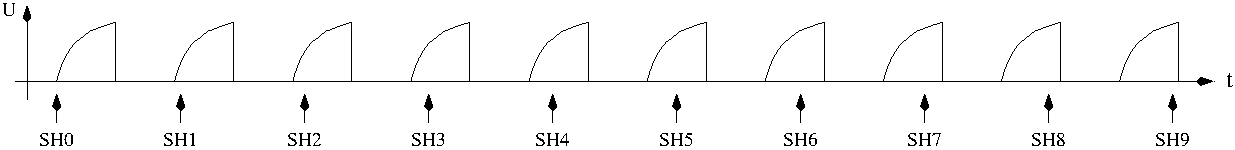
\includegraphics[width=1.\textwidth]{../FIG/sampling.pdf}
\caption{Сканирование сигналов напряжения с помощью метода выборки}
\label{fig:sampling}
\end{figure}

Одна проблема состоит в том, чтобы синхронизировать точное начало сигнала с непрерывными
тактовыми импульсами процессора.
Только триггер внешнего сигнала может сбросить делитель тактовых импульсов АЦП.
Если бы АЦП запускался программной инструкцией, делитель тактовых импульсов возобновил бы деление с начала.
Только программа, написанная на языке ассемблера, может точно определять моменты времени для этой техники 
выборки. Каждый такт микроконтроллера важен для построения программных циклов.
Анализируя характеристику напряжения при зарядке небольшого конденсатора, Вы можете видеть, что постоянная
времени не является непрерывной во время периода выборки.
Это было показано Pieter-Tjerk на презентации в \inquotes{60. UKW-Tagung in Weinheim}.
Внутренний конденсатор около \(10~pF\), который удерживает входное напряжение для преобразования,
отсоединяется в SH-время и снова подключается через два тактовых цикла АЦП.
Кроме того, есть небольшие задержки данных через полтора цикла до повторного подсоединения,
которые, вероятно, связаны с переключением мультиплексора.
Оба момента учитываются при обработке данных программным обеспечением.
Программное обеспечение выборки может обрабатывать до 255 тактов сигнала. Программное обеспечение
также может вычислять среднее значение из 32 последовательностей зарядки. Посредством построения
среднего значения эффект шума будет меньше.
Программное обеспечение выборки может контролировать и обрабатывать как заряд, так и
разряд конденсатора.
Поскольку оба направления используются для измерения величины ёмкости диода в обратном направлении,
задача калибровки измеряет значение нулевой ёмкости в обоих направлениях для всех комбинаций контактов.
Измеряя величину ёмкости диода в обоих направлениях заряда, можно показать разницу между обоими значениями.
При зарядке величина ёмкости измеряется вблизи напряжения \(0~V\), а при разряде ёмкость измеряется
вблизи напряжения \(5~V\).
Для измерения обычного конденсатора нет разницы в значениях ёмкости с такой небольшой разностью потенциалов,
которую можно обнаружить.
Поэтому для измерения малых ёмкостей используется только направление заряда (\textless 100~pF).
Pieter-Tjerk оптимизировал свою функцию для работы с тактовой частотой \(16~MHz\).
В этой конфигурации Вы получите разрешение \(0.01~pF\).
Для работы с частотой \(8~MHz\) АЦП будет работать на частоте в два раза меньше, чтобы
получить вышеупомянутые уровни напряжения сигнала в тех же точках, что и при работе на частоте \(16~MHz\).
Потеря разрешения с частотой \(8~MHz\) будет неактуальной для большинства пользователей,
а дополнительное время тестирования более медленным АЦП в этом режиме тоже допустимо.

\subsection{Измерение эквивалентного сопротивления ESR}
Эквивалентное последовательное сопротивление \(ESR\) \cite{ESR} является, к примеру, хорошим индикатором старения электролитических конденсаторов.
Рисунок~\ref{fig:Cap_equiv} показывает эквивалентную схему конденсатора.
Резистор \(Rp\) - сопротивление утечки конденсатора, \(ESL\) - эквивалентная последовательная индуктивность и
\(ESR\) представляет собой эквивалентное последовательное сопротивление.

\begin{figure}[H]
  \centering
    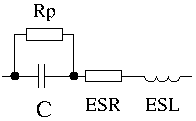
\includegraphics[width=.8\textwidth]{../FIG/Cap_equiv.pdf}
  \caption{Эквивалентная схема конденсатора}
  \label{fig:Cap_equiv}
\end{figure}

Обычно, значение \(ESR\) документируется для частоты испытания \(100~kHz\) при температуре 
\(20^{\circ} C\).
Рисунки~\ref{fig:Cap_FC_data} и \ref{fig:Cap_FR_data} показывают значения \(ESR\) конденсаторов производства 
Panasonic серий FC и \inquotes{low ESR} FR.
Обе серии способны работать до температуры \(105^{\circ} C\).
На рисунке~\ref{fig:Cap_FC_FR_data} приведены данные обеих серий с допустимым рабочим напряжением \(25~V\).
Если в ряде имеются различные типы той же ёмкости и диапазона напряжения, то для диаграммы выбраны 
с самым низким значением \(ESR\).
Значение ёмкости и \(ESR\) электролитических конденсаторов значительно отличается в зависимости от рабочей температуры. 

\begin{figure}[H]
  \centering
    \includegraphics[width=.8\textwidth]{../GNU/Cap_FC_dataRU.pdf}
  \caption{Документированное значение ESR серии FC Panasonic}
  \label{fig:Cap_FC_data}
\end{figure}

\begin{figure}[H]
  \centering
    \includegraphics[width=.8\textwidth]{../GNU/Cap_FR_dataRU.pdf}
  \caption{Документированное значение ESR серии FR Panasonic}
  \label{fig:Cap_FR_data}
\end{figure}

\begin{figure}[H]
  \centering
    \includegraphics[width=.8\textwidth]{../GNU/Cap_FC_FR_dataRU.pdf}
  \caption{Сопоставление значений ESR серий FC и FR}
  \label{fig:Cap_FC_FR_data}
\end{figure}

Нет простого способа измерить \(ESR\) на частоте \(100~kHz\) с использованием ATmega,
потому что ни АЦП не может работать на столь высокой частоте входного сигнала, ни существующая схема
не может поддерживать сигнал с частотой \(100~kHz\).
Ниже описаны два метода измерения \(ESR\), которые возможны в существующей схеме.
Оба метода используют прямоугольный сигнал для измерения. Результаты никогда не будут такими же, как 
при измеренных синусоидальным сигналом.
В первом методе измеренные значения близки к тем значениям, которые проводятся сигналом частотой \(1~kHz\).
Но второй способ имеет преимущество в том, что нулевое значение может быть определено с закороченными 
тестовыми площадками.
Кроме того, измеренное значение \(ESR\) более близко к значению, измеренному сигналом \(10~kHz\).
В настоящее время мне не известно метода измерения, который может определить значение \(ESR\), близкое к 
результату измерения \(100~kHz\).
В таблице~\ref{tab:capESR} показана зависимость результатов \(ESR\) от измеряемой частоты.
Все конденсаторы, кроме \(47~\mu F\), серии FC производства Panasonic.
Эталонные значения измерены PeakTech 2170 LCR измерителем.
Все результаты TransistorTester измерялись методом 2 \ref{sec:ESR2}.
Конденсаторы большой ёмкости трудно измерить с использованием измерительной частоты \(100~kHz\)
из-за влияния индуктивности (\(ESL\)) на результаты измерения.

\begin{table}[H]
  \begin{center}
    \begin{tabular}{| l | c | c | c | c | c |}
   \hline
            &Документация& PeakTech  & PeakTech & PeakTech & Transistor- \\
 Ёмкость    & 100 kHz    & 100 kHz   & 10 kHz   & 1 kHz    & Tester  \\
    \hline
    \hline
1uF / 50V    & 2,4       & 1,27      & 1,75     & 4,31     &  2,1 \\
    \hline
2,2uF / 50V  & 1,8       & 1,07      & 1,34     & 2,76     &  1,6 \\
    \hline
4,7uF / 50V  & 1,3       & 1,19      & 1,40     & 2,37     &  1,5 \\
    \hline
4,7uF / 50V  & 1,3       & 1,19      & 1,40     & 2,37     &  1,5 \\
    \hline
10uF / 50V   & 1,3       & 1,26      & 1,45     & 2,05     &  1,5 \\
    \hline
22uF / 10V   & 2,0       & 1,52      & 1,76     & 2,24     &  1,9 \\
    \hline
47uF / 63V   & ?         & 0,46      & 0,50     & 0,63     &  0,52 \\
    \hline
    \end{tabular}
  \end{center}
  \caption{Значения ESR различных электролитических конденсаторов}
  \label{tab:capESR} 
\end{table}

\subsection{Измерение ESR, первый метод}
Если ёмкость измеряемого конденсатора будет больше, чем \(0,45~\mu F\), то Тестер будет измерять 
также последовательное сопротивление. 
Для значения больше, чем \(3,6~\mu F\) используется нормальная тактовая частота для АЦП – \(125~kHz\). 
Для более низких значений ёмкости, чтобы ускорить измерение, используется более высокая тактовая частота - \(500~kHz\). 
Точность результатов АЦП будет выше с более высокой тактовой частотой, но это может привести к высоким значениям 
ESR конденсаторов с более низкой величиной ёмкости. Иначе измерение ESR этим методом будет невозможно для значений 
меньше, чем \(1,8~\mu F\) при нормальной тактовой частоте \(125~kHz\).

Строго говоря, ESR конденсатора зависит от частоты и температуры. Обычно в технических описаниях приведена величина, 
измеренная на синусоидальном сигнале частотой \(100~kHz\). Такое измерение не может быть сделано ATmega без внешнего 
оборудования. Описанная ниже методика, основанная на стандартной тактовой частоте АЦП, использует для измерения 
практически прямоугольный сигнал частотой ниже \(640~Hz\). С тактовой частотой АЦП \(500~kHz\) частота измерения 
будет \(2400~Hz\). Чтобы получить величину ESR, будет измерено напряжение на обоих выводах конденсатора во время 
зарядки в одном направлении с внутренним опорным напряжением АЦП (\(1,1~V\)). После измерения ток зарядки будет отключен, 
и напряжение на конденсаторе будет измерено снова без тока. Если это напряжение ниже \(3~mV\), последовательность 
измерения будет повторена. На рисунке~\ref{fig:Cap_esr} представлены соответствующие схемы.
 
\begin{figure}[H]
 \centering
  \begin{overpic}[width=.83\textwidth]{../FIG/Cap_esr.pdf}
   \color{black}
   \put(28,85){\makebox(0,0)[cb]{Voltage measurement with charge current}}
   \put(28,40){\makebox(0,0)[cb]{Voltage measurement without current}}
  \end{overpic}
 \caption{Схема измерения ESR конденсатора}
 \label{fig:Cap_esr}
\end{figure}

Разница напряжения на конденсаторе с током и без тока пропорциональна внутреннему сопротивлению конденсатора. 
Ожидаемое напряжение этой разницы настолько мало, что одно измерение не может привести к удовлетворительному 
результату. Поэтому ток будет переключен на противоположное направление, и будет повторено то же самое измерение. 
Измерения будут проведены последовательно 128 раз, и результаты измерений напряжения будут суммироваться. Таким 
образом, у нас будут 3 суммы напряжений: напряжение \(Ulp\) с низкой стороны конденсатора с током, напряжение \(Uhp\) 
с высокой стороны конденсатора с током и напряжение \(Uc\) с высокой стороны конденсатора без тока. Сумма напряжений 
с низкой стороны конденсатора представляет собой падение потенциала при зарядке на выходном сопротивлении 
порта \(Rport\). 
Разница напряжений с высокой  и низкой сторон конденсатора представляет напряжение на конденсаторе при 
зарядке \(Udiff = Uhp - Ulp\). Разница \(Uesr = Udiff - Uc\) должна представлять падение напряжения на внутреннем 
сопротивлении конденсатора при зарядке. Вычисляем величину сопротивления как отношение напряжения \(Uesr\) к 
напряжению \(Ulp\), измеренному при известной величине выходного сопротивления порта \(Rport\).
Коэффициент пропорциональности выбран так, чтобы получить разрешение 
сопротивления \(0,01~\Omega\):  \(Resr = \frac{Uesr \cdot 10 \cdot Rport}{Ulp}\)
Рисунок~\ref{pic:esr4} показывает часть кривой напряжения на конденсаторе \(4,2~\mu F\) во время измерения ESR. 
Чтобы пояснить влияние ESR, к конденсатору добавлен последовательный резистор \(6,8~\Omega\).
Кратковременное отключение напряжения после зарядки конденсатора интерпретируется программным обеспечением, 
как переход к измерению ESR. Большее падение напряжения к потенциалу GND во время измерения вызвано выходным 
сопротивлением порта около \(20~\Omega\).
При этом измерении Тестер выводит на дисплей полную величину ESR \(7,5~\Omega\). Вычитая величину последовательного 
резистора \(6,8~\Omega\), получим ESR \(0,56~\Omega\).
На рисунке~\ref{pic:esr2} представлена диаграмма измерения электролитического конденсатора \(2,2~\mu F\) с 
ESR \(6,5~\Omega\) на более высокой частоте измерения.


\begin{figure}[H]
  \begin{subfigure}[b]{.5\textwidth}
    \centering
    \includegraphics[width=1.\textwidth]{../PNG/ESR_4uF.png}
    \caption{measured one pin to GND}
  \end{subfigure}
  ~
  \begin{subfigure}[b]{.5\textwidth}
    \centering
    \includegraphics[width=1.\textwidth]{../PNG/ESR4uF6R8.png}
    \caption{measured pin to pin}
  \end{subfigure}
  \caption{Кривая напряжения во время измерения ESR конденсатора \(4,2~\mu F\)}
  \label{pic:esr4}
\end{figure}


\begin{figure}[H]
  \begin{subfigure}[b]{.5\textwidth}
    \centering
    \includegraphics[width=1.\textwidth]{../PNG/ESR_2uF_pin2GND.png}
    \caption{measured one pin to GND}
  \end{subfigure}
  ~ 
  \begin{subfigure}[b]{.5\textwidth}
    \centering
    \includegraphics[width=1.\textwidth]{../PNG/ESR_2uF_pin2pin.png}
    \caption{measured pin to pin}
  \end{subfigure}
  \caption{Кривая напряжения во время измерения ESR конденсатора \(2,2~\mu F\)}
  \label{pic:esr2}
\end{figure}


Точность измерения ESR не высока по нескольким причинам:
\begin{enumerate}
\item Измерение напряжения на обоих выводах конденсатора не может быть сделано одновременно, а только последовательно. 
В промежутке между обоими измерениями ток зарядки изменяется из-за заряда конденсатора. Программа пытается 
компенсировать этот  факт коррекцией ёмкости в зависимости от напряжения низкой стороны.
\item АЦП начинает измерять напряжение с задержкой на 1,5 тактовых импульса с начала преобразования. Преобразование 
начинается по переднему фронту тактовой частоты АЦП, если установлен стартовый бит. Если ток зарядки будет отключен 
раньше, то АЦП зафиксирует неправильное напряжение для измерения с током. Если ток зарядки будет отключен позже, 
конденсатор получит больший электрический заряд, чем при надлежащем измерении с током зарядки. Это даст слишком 
высокое измеренное  напряжение без тока. Выключение тока в нужное время представляет трудности для программного 
обеспечения.
\item В качестве опорной величины для измерения этим методом используется выходное сопротивление порта, которое 
точно не известно. 
\item Разрешение АЦП недостаточно, чтобы получить разрешение сопротивления \(0,01~\Omega\).
Для  лучшего разрешения АЦП для всех измерений используется внутренний ИОН (\(1,1~V\)). Разрешение также увеличивается 
за счет большего числа одиночных измерений.
\item Переключение портов не может быть точно синхронизировано с тактовой частотой АЦП после опроса завершения 
преобразования.
\end{enumerate}

Тем не менее, как показано на следующем рисунке~\ref{fig:Cesr}.
результаты оказываются практичными. Значения ESR, того же самого элемента, измеренные Тестером, различаются больше, 
чем величины, измеренные LCR-метром. Значения ESR замерены LCR метром на частоте \(1~kHz\) или интерполированы для 
небольших конденсаторов на частоту \(2,4~kHz\). Вы должны учитывать качество всех соединителей. Используемые 
кабельные соединения могут увеличить измеренное значение сопротивления. Разъёмы также могут увеличить значение 
сопротивления. В LCR-метре используется зажимы Кельвина, что дает преимущество при измерении. Только один конденсатор 
в серии испытаний ниже \(1~\mu F\) на \(500~nF\) был керамическим, все остальные были пленочными конденсаторами. 
Единственным электролитическим конденсатором в серии испытаний ниже \(9~\mu F\) был конденсатор на \(2,2~\mu F\).

\begin{figure}[H]
\centering
\includegraphics[width=.93\textwidth]{../GNU/CesrRU.pdf}
\caption{Результаты измерений ESR 15-ти различных ATmega}
\label{fig:Cesr}
\end{figure}


\subsection{Измерение ESR, второй метод}
\label{sec:ESR2}
Начиная с версии 1.07k программного обеспечения, применен новый метод измерения ESR. Последовательные шаги измерения 
показаны на рисунке ~\ref{fig:Cap_esr2}. Отличие от предыдущего метода в том, что длительность протекания тока через 
конденсатор существенно короче. Конденсатор предварительно заряжен половиной импульса в отрицательном направлении и 
циклически перезаряжается в обоих направлениях. Время  импульса зарядки выбрано так, что отсчёты проводят в середине 
импульсов зарядки отсчётов 4 и 8 и синхронизируют в это время АЦП (2.5 тактовых импульса после начала преобразования 
АЦП). Полный цикл измерения показан на рисунке~\ref{fig:Cap_esr2_timing}.
Сумма результатов 255 циклов измерения используется для того, чтобы получить результат с соответствующим разрешением. 
Продолжением зарядки конденсатора в любом направлении избегают ту же зарядку и разрядку длительным импульсом в той 
же схеме. При измерении опорного напряжения конденсатор остается обесточенным. Тем самым время измерения не критично. 
Предполагается только, что захват напряжения конденсатора производится до начала следующего импульса зарядки или 
разрядки. 

\begin{figure}[H]
  \centering
    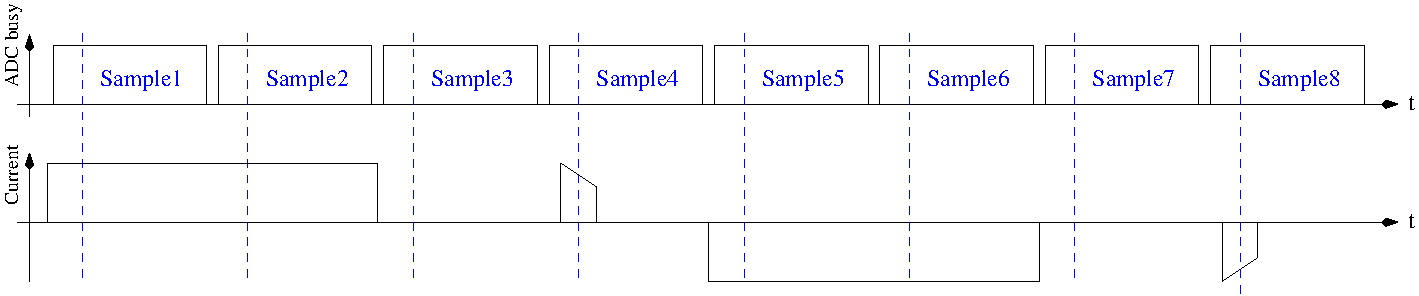
\includegraphics[width=1.\textwidth]{../FIG/Cap_esr2_timing.pdf}
  \caption{Временная диаграмма цикла измерения для нового способа измерения ESR}
  \label{fig:Cap_esr2_timing}
\end{figure}

\begin{figure}[H]
 \centering
  \begin{overpic}[width=.83\textwidth]{../FIG/Cap_esr2.pdf}
   \color{black}
   \put(20,98){\makebox(0,0)[cb]{Forward reference measurement}}
   \put(20,72){\makebox(0,0)[cb]{Forward voltage measurement with probe current}}
   \put(20,47){\makebox(0,0)[cb]{Reverse reference measurement}}
   \put(20,21){\makebox(0,0)[cb]{Reverse voltage measurement with probe current}}
  \end{overpic}
 \caption{Более простое измерение ESR конденсатора}
 \label{fig:Cap_esr2}
\end{figure}


Из-за более короткого импульса зарядки может быть измерено не только ESR конденсаторов с более низкой ёмкостью, но 
этот способ измерения может также использоваться для измерения резисторов с небольшим сопротивлением, если у них нет 
обнаруженной индуктивности. Этим методом для таких  резисторов может быть достигнуто разрешение \(0,01~\Omega\). Этим 
же методом может быть откалибровано нулевое сопротивление для всех трех комбинаций испытательных выводов в режиме 
самопроверки. Вы должны иметь в виду, что для устойчивых результатов нужны качественные разъемы и зажимы. Период 
измерения около \(900~\mu s\), что соответствует частоте приблизительно \(1,1~kHz\).
Поскольку импульс зарядки очень короток, результат измерения сопоставим с измерениями на частоте \(10~kHz\).
Пример измерения плёночного конденсатора ёмкостью \(10~\mu F\) проведенным с ним одним и с включенным последовательно 
с ним резистором на \(2,7~\Omega\), 
показан на  рисунке~\ref{pic:NewEsr10}.
Вы можете видеть эффект дополнительного сопротивления, сравнивая обе осциллограммы. Вы можете видеть также, почему 
измерение АЦП (SH) должно приходиться на середину импульса зарядки. При больших значениях ёмкости ток зарядки  почти 
устойчив во время всей длительности импульса: таким образом, Вы получите среднее напряжение в середине импульса 
зарядки. С более низкими значениями ёмкости Вы получите существенную  разницу, которая  может быть cкомпенсирована 
для известной величины ёмкости.

\begin{figure}[H]
  \begin{subfigure}[b]{.5\textwidth}
    \centering
    \includegraphics[width=1.\textwidth]{../PNG/NewEsr10uF0R0.png}
    \caption{без последовательного сопротивления}
  \end{subfigure}
  ~
  \begin{subfigure}[b]{.5\textwidth}
    \centering
    \includegraphics[width=1.\textwidth]{../PNG/NewEsr10uF2R7.png}
    \caption{с последовательным сопротивлением \(2,7~\Omega\)}
  \end{subfigure}
  \caption{Кривая напряжения при новом измерении ESR конденсатора \(10~\mu F\)}
  \label{pic:NewEsr10}
\end{figure}

При использовании импульса длительностью \(27~\mu s\) можно определить ESR для конденсаторов ёмкостью больше \(180~nF\).
Для измерения конденсаторов с низкой ёмкостью, в версии 1.11k импульс сокращается до \(8~\mu s\).
Рисунок~\ref{pic:NewEsr2} показывает кривую напряжения на конденсаторе \(2,2~\mu F\) с 
последовательно подключенным сопротивлением \(2,7~\Omega\) и без него.

\begin{figure}[H]
  \begin{subfigure}[b]{.5\textwidth}
    \centering
    \includegraphics[width=1.\textwidth]{../PNG/NewEsr2u2F0R0.png}
    \caption{без последовательного сопротивления}
  \end{subfigure}
  ~
  \begin{subfigure}[b]{.5\textwidth}
    \centering
    \includegraphics[width=1.\textwidth]{../PNG/NewEsr2u2F2R7.png}
    \caption{с последовательным сопротивлением \(2,7~\Omega\)}
  \end{subfigure}
  \caption{Кривая напряжения измерения~ESR конденсатора \(2,2~\mu F\) зарядным импульсом \(8~\mu s\)}
  \label{pic:NewEsr2}
\end{figure}

На рисунке~\ref{pic:NewEsr2} не видно момент измерения ADC. 
На рисунке~\ref{pic:NewEsr2zoom} изображена кривая напряжения в увеличенном масштабе. 
Момент измерения совпадает с срединой рисунка.

\begin{figure}[H]
  \begin{subfigure}[b]{.5\textwidth}
    \centering
    \includegraphics[width=1.\textwidth]{../PNG/NewEsr2u2F0R0zoom.png}
    \caption{без последовательного сопротивления}
  \end{subfigure}
  ~
  \begin{subfigure}[b]{.5\textwidth}
    \centering
    \includegraphics[width=1.\textwidth]{../PNG/NewEsr2u2F2R7zoom.png}
    \caption{с последовательным сопротивлением \(2,7~\Omega\)}
  \end{subfigure}
  \caption{Увеличенная кривая напряжения на конденсаторе \(2,2\mu F\) при измерении~ESR зарядным импульсом \(8 \mu s\)}
  \label{pic:NewEsr2zoom}
\end{figure}


Результаты измерений по новому методу измерения ESR показаны на рисунке~\ref{fig:Cesr2}.
Значения ESR отличаются от результатов, показанных для предыдущего метода измерения на рисунке~\ref{fig:Cesr} потому 
что ESR зависит от частоты. Эталонные значения определены  LCR-метром на частоте измерения \(10~kHz \).

\begin{figure}[H]
\centering
\includegraphics[width=.93\textwidth]{../GNU/Cesr2RU.pdf}
\caption{Результаты измерения ESR методом 2 15-ю различными ATmega}
\label{fig:Cesr2}
\end{figure}

Ряд измерений различных электролитических конденсаторов показан на рисунке~\ref{fig:ElcoESR}.
Вместе с результатами Тестера представлены результаты измерений LCR метра PeakTech 3315 на различных частотах. На 
этой диаграмме сопротивление представлено в логарифмическом масштабе. Во всех случаях результаты Тестера близки к 
результатам измерений LCR метра на частоте \(10~kHz\). Из тестируемых, только конденсатор \(500~\mu F~/~3~V\) - более 
старый образец, все остальные конденсаторы - новые.

\begin{figure}[H]
\centering
\includegraphics[width=.93\textwidth]{../GNU/Elco_esrRU.pdf}
\caption{Результаты измерений ESR различных электролитических конденсаторов}
\label{fig:ElcoESR}
\end{figure}


Новый метод измерения может быть использован для измерения резисторов с низким сопротивлением. Погрешности измерения 
некоторых резисторов ниже \(10~\Omega\) с тремя примерами каждого типа ATmega показаны на рисунке~\ref{fig:res_esr}. 

\begin{figure}[H]
\centering
\includegraphics[width=1.\textwidth]{../GNU/res_esrRU.pdf}
\caption{Погрешность измерения сопротивления методом ESR}
\label{fig:res_esr}
\end{figure}

С программным обеспечением версии 1.12k длительность импульса заряда конденсатора уменьшается до \(2~\mu s\) для
возможности измерения ESR конденсаторов с более низкими значениями ёмкости. Теперь можно измерить значение ESR
для конденсаторов от \(20~nF\).
Но ошибка измерения будет расти при меньших значениях ёмкости. Причиной этого является уменьшение постоянной времени
RC-цепочки, которая будет только \(14.4~\mu s\) для значения ёмкости \(20~nF\).
Это приведет к быстрому изменению напряжения на конденсаторе при импульсе в \(2~\mu s\) тока.
Программное обеспечение может выбрать дискретизацию АЦП только в один такт процессора.
Но входной АЦП имеет постоянную времени, примерно \(0.24~\mu s\), которая может варьироваться в зависимости
от экземпляра ATmega.
Эти вариации постоянной времени фильтра входного АЦП не могут быть отслежены программным обеспечением.
Время выборки АЦП недоступно за долю периода тактовой частоты.
При большем значении ёмкости измеряемого конденсатора постоянная времени будет расти и изменение напряжения 
при импульсе тока будет уменьшаться. По этой причине, изменение постоянной времени фильтра входного АЦП 
оказывает меньший эффект при измерении конденсатора с большей ёмкости.
На рисунке~\ref{pic:Cesr_22n} показаны результаты для некоторых конденсаторов при измерении на 10 различных тестерах.
На изображении слева - результаты ESR некоторых конденсаторов имеют более высокие значения ESR.
Результаты довольно похожи в сравнении с результатами тестера LCR Peaktech 2170 при \(10~kHz\) и при \(100~kHz\).
На рисунке справа Вы можете увидеть результаты измерений некоторых высококачественных конденсаторов с низким значением ESR.
Хотя и заметен предел метода (особенно при низких значениях ёмкости), но это лучше, чем полное отсутствие информации.
В любом случае, Вы можете сравнить несколько конденсаторов одинаковой ёмкости с малыми значениями для поиска 
более качественного экземпляра.

\begin{figure}[H]
  \begin{subfigure}[b]{.5\textwidth}
    \centering
    \includegraphics[width=1.\textwidth]{../GNU/Cesr_22nRU.pdf}
    \caption{высокое значение ESR}
  \end{subfigure}
  ~
  \begin{subfigure}[b]{.5\textwidth}
    \centering
    \includegraphics[width=1.\textwidth]{../GNU/Cesr_22n_lowRU.pdf}
    \caption{низкое значение ESR}
  \end{subfigure}
  \caption{Измерения ESR конденсаторов малой ёмкости}
  \label{pic:Cesr_22n}
\end{figure}


Для микроконтроллеров с объемом флеш памяти более 16~K в программном обеспечении 1.12k резистор \(470~k\Omega\) 
для половины измерений подключается параллельно резистору \(680~\Omega\) с целью небольшого увеличения тока при измерении.
К сожалению, увеличение тока незначительное, чтобы полученное в результате изменение напряжения изменило результат АЦП.
Увеличение напряжения составляет лишь около 20~\% от разрешения АЦП при использовании ИОН \(1.1~V\).
Для изменения отдельных значений предпочтительнее было бы добавление незначительного шума на вход АЦП.
С помощью этой функции можно достичь статистического улучшения разрешения АЦП путем усреднения результатов измерений.


\subsection{Потеря напряжения после импульса зарядки, Vloss}
Для конденсаторов большой ёмкости, была проанализирована потеря напряжения на конденсаторе после того, как он был 
заряжен. Достигнутое напряжение заряда на  электролитических конденсаторах терялось после короткого периода. Эта 
потеря напряжения могла быть вызвана параллельно подключенным резистором. Но я принимаю, что эта потеря напряжения 
электролитических конденсаторов вызвана внутренним рассеиванием заряда непосредственно после импульса зарядки. 
Заряжая конденсаторы через резистор \(470~k\Omega\), как это сделано для небольших ёмкостей, это рассеивание 
проявляется сразу после выключения тока. Но в этом случае никакая потеря напряжения не была обнаружена. Но если 
Вы заряжаете тот же самый конденсатор с более низкой ёмкостью коротким импульсом тока, то также обнаружите потерю 
напряжения на конденсаторе. Тот же самый эффект, с более низкой потерей, может также быть замечен для керамических 
конденсаторов. Я заметил, что конденсаторы с потерей напряжения более, чем на несколько \%, весьма вероятно, имеют 
низке качестве. Особенно заметна относительная потеря напряжения у более старых бумажных конденсаторов, у которых 
замечены проблемы и при других измерениях. Некоторые примеры измерений показаны  в таблице.

\begin{tabular}{| l | c | c | c | c | c | c |}
   \hline
Тип           & Величина      & PeakTech      & Voltcraft & PeakTech & Transistor- \\
конденсатора & ёмкости & LCR 2170     & M2650-B   &  3315    & Tester      \\
    \hline
    \hline
бумажный     & 4700pF      & 6,75-10,36nF & 8,00nF    &  25,40nF & 10,71nF  \\
          &             & Q=2,5-32     &           &          & Vloss=11\% \\
    \hline
бумажный     & 6800pF      & 9,40-11,40nF & 10,41nF   &  23,30nF & 11,65nF \\
          &             & Q=5-25       &           &          & Vloss=5,0\% \\
    \hline
неизвестный  & 4700pF      & 5,85-6,33nF & 6,12nF    &  6,90nF  & 6225pF \\
           &             & Q=16-87     &           &          & Vloss=1,7\% \\
    \hline
фольговый      & 7870pF      & 7,86-7,87nF  & 7,95nF    &  7,95nF  & 7872pF \\
          &             & Q= \textgreater~1540     &           &          & Vloss=0\% \\
    \hline
бумажный     & 22000pF     & 37,4-57,5nF  & 52,8nF    &  112nF   & 118,5nF \\
          &             & Q=2,5-32     &           &          & Vloss=12\% \\
    \hline
фольговый      & 22600pF     & 22,4-22,5nF  & 22,57nF   & 22,69nF  & 22,54nF \\
          &             & Q= \textgreater~1540     &           &          & Vloss=0\% \\
    \hline
бумажный     & 100nF       & 144-256nF    & 177nF     &  318nF   & 529,7nF \\
          &             & Q=2,6-28     &           &          & Vloss=12\% \\
    \hline
керамический & 100nF       & 97,7-102nF   & 103,7nF   & 103,3nF  & 103,1nF \\
          &             & Q=90-134     &           &          & Vloss=0,1\% \\
    \hline
фольговый      & 100nF       & 98,0-101nF   & 101,4nF   & 102,2nF  & 101,6nF \\
          &             & Q=58-700     &           &          & Vloss=0\% \\
    \hline
\end{tabular}

В этой таблице Вы видите, что ёмкость всех фольговых конденсаторов может быть измерена всеми приборами с хорошей 
точностью. Значение ёмкости и добротности (Q)  PeakTech LCR-метра являются минимальными и максимальными значениями 
измерений в частотном диапазоне от \(100~Hz\) до \(100~kHz\).
Во всех примерах в таблице потеря напряжения Vloss, замеренная Тестером, велика, если конденсаторы низкокачественные. 
Только в этих случаях различие результатов измерения ёмкости также большие. Тестер может определить потерю напряжения, 
если измеренное значение ёмкости больше \(5000~pF\).

\subsection{Отдельное измерение ёмкости и ESR}
Отдельное измерение ёмкости с последующей оценкой ESR можно выбрать из диалогового меню дополнительных функций
только для ATmega с достаточным объемом памяти. Этот тип измерения предназначен для тестирования конденсаторов
без демонтажа.
Пожалуйста, убедитесь, что все конденсаторы на плате разряжены, прежде чем начать измерение!
Испытание установленных в плату копонентов производится низким, насколько это возможно,
напряжением, лишь немного больше \(300~mV\).
Кроме того, измерение производится с использованием только резистора \(680~\Omega\) для 
уменьшения влияния связанных компонентов печатной платы.
Для определения конденсаторов малых ёмкостей, измерение начинается с коротких импульсов 
зарядки \(200~\mu s\). Если заряд конденсатора короткими импульсами не достигнет \(300~mV\) 
за \(2~ms\), то последующий заряд осуществляется импульсами \(2~ms\).
Когда ёмкость измеряемого конденсатора большая, напряжение заряда импульсами \(2~ms\) увеличивается медленно,
то, в этом случае, ширина импульса(ов) заряда увеличится до \(20~ms\).
Если напряжение на измеряемом конденсаторе приближается к \(300~mV\), снова используются
короткие импульсы заряда.
Общее время импульсов суммируется после достижения напряжения заряда больше \(300~mV\),
ёмкость вычисляется по времени и уровню заряда конденсатора.
С помощью этого метода возможно измерение ёмкости чуть ниже от \(2~\mu F\). Верхний предел измеряемой ёмкости
ограничен временем заряда \(2,5~s\), примерно \(50~mF\).
После успешного измерения ёмкости, измеряется ESR конденсатора по описанному 
в разделе~\ref{sec:ESR2} методу.
Результат кратковременно отображается на дисплее, а затем сразу же начинается следующее измерение.        
Измерения останавливаются после серии из 250 измерений или по нажатию кнопки \textbf{ TEST},
после чего программа возвращается в диалоговое меню дополнительных функций.



\subsection{Результаты измерения ёмкости конденсаторов}
Результаты моих измерений ёмкости для трех микроконтроллеров ATmega8 показаны на рисунке~\ref{fig:mega8cap}. Некоторые 
значения оригинального программного обеспечения показаны с поправочным коэффициентом 0,88 (-12\%).
Другие результаты измерения различных версий ATmega8 показаны на рисунках~\ref{fig:mega8Acap} и \ref{fig:mega8Lcap}.
Результаты измерения тех же самых конденсаторов для ATmega168 показаны на рисунке~\ref{fig:mega168cap}.
Основой для вычисления погрешности являются результаты измерения немаркированных элементов LCR метром PeakTech 2170. 
Часть относительно большой разницы измерений вызвана слишком высокой частотой измерения LCR-метра для больших 
электролитических конденсаторов. С другой стороны плохое качество электролитических конденсаторов может дать другой 
процент.

\begin{figure}[H]
\centering
\includegraphics[width=.93\textwidth]{../GNU/Mega8capRU.pdf}
\caption{Погрешность измерения ёмкости в \% с ATmega8 }
\label{fig:mega8cap}
\end{figure}

\begin{figure}[H]
  \begin{subfigure}[b]{.5\textwidth}
    \centering
    \includegraphics[width=1.\textwidth]{../GNU/Mega8AcapRU.pdf}
    \caption{ATmega8A}
    \label{fig:mega8Acap}
  \end{subfigure}
  ~
  \begin{subfigure}[b]{.5\textwidth}
    \centering
    \includegraphics[width=1.\textwidth]{../GNU/Mega8LcapRU.pdf}
    \caption{ATmega8L}
    \label{fig:mega8Lcap}
  \end{subfigure}
  \caption{Относительная погрешность измерения ёмкости}
\end{figure}

\begin{figure}[H]
\centering
\includegraphics[width=1.\textwidth]{../GNU/Mega168capRU.pdf}
\caption{Погрешность измерения ёмкости в \% с ATmega168 }
\label{fig:mega168cap}
\end{figure}

Рисунок~\ref{fig:capcompare} иллюстрирует, как сложно выбрать правильный алгоритм для измерения ёмкости. Все 
результаты измерения сравниваются с лучшими оценочными значениями ёмкости. Линия графика \inquotes{Мультиметр} показывает 
отличие от результатов мультиметра PeakTech 3315. Следующая линия графика \inquotes{LCR} показывает различие результатов 
PeakTech 2170 LCR-метра, который выбран из-за лучшего приближения по частоте измерения. Для сравнения этих 
результатов с результатами Тестера на ATmega168 показана линия графика \inquotes{ATmega168as}. Я уверен, что эти погрешности 
не являются реальными ошибками измерения конкретного оборудования потому, что лучшее оценочное значение также не 
соответствует реальному значению ёмкости конденсаторов.

\begin{figure}[H]
\centering
\includegraphics[width=1.\textwidth]{../GNU/capcompareRU.pdf}
\caption{Сравнение результатов измерений ёмкости мультиметром, LCR-метром и Тестером на ATmega168}
\label{fig:capcompare}
\end{figure}

В этом случае результаты LCR-метра взяты в качестве базы для сравнения. Те же самые результаты для трех различных 
микроконтроллеров ATmega168 показаны на рисунке~\ref{fig:mega168all}, микроконтроллеров ATmega168A показаны на 
рисунке~\ref{fig:mega168Aall}, для микроконтроллеров ATmega168PA - на рисунке~\ref{fig:mega168PAall}.
Результаты трех ATmega328 дополнительно показаны на рисунке~\ref{fig:mega328all}, а трех ATmega328P - на 
рисунке~\ref{fig:mega328Pall}.
В них учтена только нулевая ёмкость измерения \(39~pF\), все другие средства, чтобы скорректировать результаты 
не используются. В эту нулевую ёмкость включена также ёмкость \(2-3~pF\), которую дает кабель с зажимами длиной 12 см. 
Разводка платы также может дать, отличное от нулевого, значение ёмкости, я зафиксировал эту нулевую ёмкость для 
платы \inquotes{DG2BRS V 5.2.1}.

\begin{figure}[H]
  \begin{subfigure}[b]{.5\textwidth}
    \centering
    \includegraphics[width=1.\textwidth]{../GNU/Mega168allRU.pdf}
    \caption{ATmega168}
    \label{fig:mega168all}
  \end{subfigure}
  ~
  \begin{subfigure}[b]{.5\textwidth}
    \centering
    \includegraphics[width=1.\textwidth]{../GNU/Mega168AallRU.pdf}
    \caption{ATmega168A}
    \label{fig:mega168Aall}
  \end{subfigure}
\caption{Погрешность измерения ёмкости, не откалиброван}
\end{figure}

\begin{figure}[H]
\centering
\includegraphics[width=.93\textwidth]{../GNU/Mega168PAallRU.pdf}
\caption{Погрешность измерения ёмкости тремя ATmega168PA, не откалиброван}
\label{fig:mega168PAall}
\end{figure}

\begin{figure}[H]
  \begin{subfigure}[b]{.5\textwidth}
    \centering
    \includegraphics[width=1.\textwidth]{../GNU/Mega328allRU.pdf}
    \caption{ATmega328}
    \label{fig:mega328all}
  \end{subfigure}
  ~
  \begin{subfigure}[b]{.5\textwidth}
    \centering
    \includegraphics[width=1.\textwidth]{../GNU/Mega328PallRU.pdf}
    \caption{ATmega328P}
    \label{fig:mega328Pall}
  \end{subfigure}
\caption{Погрешность измерения ёмкости, не откалиброван}
\end{figure}

Чтобы получить лучшую точность, Вы должны приспособить программное обеспечение к индивидуальной особенности Вашего 
образца ATmega. Для этого Вы можете установить напряжение коррекции REF\_C\_KORR для компаратора, который будет 
использоваться для измерения небольших ёмкостей. Коррекция в \(1~mV\) уменьшает результаты измерения на  o 0.11~\% .
Для больших ёмкостей Вы можете определить значение C\_H\_KORR, показывающее, насколько превышены измеренные величины 
ёмкости. Поскольку конденсаторы  большой ёмкости в большинстве электролитические конденсаторы с худшим качеством, 
измерение их ёмкости осложнено. Это также дополнительно усложняет дифференцирование отличий от реальных значений 
ёмкости.

Я заметил, особенно с микроконтроллерами ATmega168, аномалию результатов измерения малых ёмкостей, которая зависит 
от скорости нарастания напряжения во время зарядки конденсатора. Рисунок~\ref{fig:mega168optcap} показывает 
погрешность измерения ёмкости, когда учитывают только нулевое значение (168-3-A), с поправочным коэффициентом для 
малых ёмкостей REF\_C\_KORR=66, также и с поправочным коэффициентом для больших ёмкостей C\_H\_ KORR=5 (168-3-B), 
плюс, дополнительно отклонение 168 3 C с моделью зависимости от скорости нарастания для измерения малых 
ёмкостей (COMP\_SLEW1=4000  и COMP\_SLEW2=220). Саморазряд больших ёмкостей  также учтен в отклонении 168-3-C. 
Элемент с зависимостью от величины скорости нарастания вычисляется 
как \(\frac{COMP\_SLEW1}{cval+COMP\_SLEW2} - \frac{COMP\_SLEW1}{COMP\_SLEW2}\),
где cval  измеренное  значение ёмкости в \(pF\).

\begin{figure}[H]
\centering
\includegraphics[width=.93\textwidth]{../GNU/Mega168cap_optRU.pdf}
\caption{Улучшенное измерение ёмкости ATmega168}
\label{fig:mega168optcap}
\end{figure}

\subsection{Автоматическая калибровка при измерении конденсаторов}

Автоматическая калибровка состоит из двух частей. Первая часть определяет смещение нуля при измерении ёмкости. 
Для этого определяется значение ёмкости, измеренной без подключенного конденсатора. Значение ёмкости для всех 6 
комбинаций измерений, определяется с 8 повторениями. После успешного определения, смещение нуля записывается в 
EEprom и будет использоваться для дальнейших измерений. Более сложным было выявление различия вариантов 
микроконтроллеров ATmega для малых конденсаторов (\textless \(40~\mu F\)),
которые показаны на рисунках ~\ref{fig:mega168all}, \ref{fig:mega168Aall} и \ref{fig:mega168PAall}.
Основной причиной  этого является различие характеристик (напряжения смещения) аналогового компаратора.

Данные  измерения девяти различных микроконтроллеров показаны на рисунке~\ref{fig:CompAdjust} .
Точки \inquotes{dif2ref} показывают разницу напряжения заряженного конденсатора \(660~nF\) с  индивидуальным внутренним 
опорным напряжениям (ширина запрещенной зоны). В идеале это различие напряжений должно быть равно нулю, если 
аналоговый компаратор остановил зарядку сигналом для микроконтроллера. Короткое время обработки микроконтроллера 
не должно заканчиваться измерением результата роста напряжения этого относительно большого конденсатора. 
Точки \inquotes{CapErr} показывают предполагаемые погрешности измерения каждого 
микроконтроллера из рисунков~\ref{fig:mega168all}, \ref{fig:mega168Aall} 
и \ref{fig:mega168PAall} с заводскими установками. Представляет интерес, как точки \inquotes{CapErr} будут соответствовать 
точкам \inquotes{dif2ref}. Для этого точки \inquotes{dif} показывают различие между соответствующими точками \inquotes{CapErr} и \inquotes{dif2ref}. 
Зная значения величин точек \inquotes{dif}, мы можем получить хорошую оценку для коррекции измерений ёмкости вместе с 
разницей между напряжением заряженного конденсатора и напряжением внутренней опоры. 

Во второй части, для внесения поправок, Вы должны подключить конденсатор к испытательным выводам 1 и 3. Этот 
конденсатор должен быть \textbf{ высококачественным} и иметь величину в диапазоне от \(100~nF\) до \(20~\mu F\).
В лучшем случае это должен быть \textbf{ плёночный конденсатор}, по возможности - \textbf{ не керамический} и ни в коем 
случае - \textbf{ не электролитический}. Точная ёмкость этого конденсатора не важна.

\begin{figure}[H]
\centering
\includegraphics[width=.8\textwidth]{../GNU/ComparatorAdjustRU.pdf}
\caption{Данные для 9 ATmega168}
\label{fig:CompAdjust}
\end{figure}

Рисунки~\ref{fig:mega168cal}, \ref{fig:mega168Acal}, \ref{fig:mega168PAcal}, \ref{fig:mega328cal} 
и \ref{fig:mega328Pcal} показывают результаты измерения различных микроконтроллеров со стандартным программным 
обеспечением после автокалибровки. Микроконтроллеры были загружены одинаковым программным обеспечением, только 
для программы avrdude в Makefile в опции \inquotes{PARTNO = }  был выбран соответствующий тип микроконтроллера (\inquotes{m168}, 
\inquotes{m168p}, \inquotes{m328} или \inquotes{m328p}). После загрузки данных была проведена самопроверка для каждого типа ATmega с 
подключением конденсатора \(330~nF\) к испытательным выводам 1 и 3 во время теста 10.

\begin{figure}[H]
  \begin{subfigure}[b]{.5\textwidth}
    \centering
    \includegraphics[width=1.\textwidth]{../GNU/Mega168calRU.pdf}
    \caption{ATmega168}
    \label{fig:mega168cal}
  \end{subfigure}
  ~
  \begin{subfigure}[b]{.5\textwidth}
    \centering
    \includegraphics[width=1.\textwidth]{../GNU/Mega168AcalRU.pdf}
    \caption{ATmega168A}
    \label{fig:mega168Acal}
  \end{subfigure}
  \caption{Погрешность измерения ёмкости, откалиброван}
\end{figure}

\begin{figure}[H]
\centering
\includegraphics[width=.93\textwidth]{../GNU/Mega168PAcalRU.pdf}
\caption{Погрешность измерения ёмкости тремя ATmega168PA, откалиброван}
\label{fig:mega168PAcal}
\end{figure}

\begin{figure}[H]
  \begin{subfigure}[b]{.5\textwidth}
    \centering
    \includegraphics[width=1.\textwidth]{../GNU/Mega328calRU.pdf}
    \caption{ATmega328}
    \label{fig:mega328cal}
  \end{subfigure}
  ~
  \begin{subfigure}[b]{.5\textwidth}
    \centering
    \includegraphics[width=1.\textwidth]{../GNU/Mega328PcalRU.pdf}
    \caption{ATmega328P}
    \label{fig:mega328Pcal}
  \end{subfigure}
  \caption{Погрешность измерения ёмкости, откалиброван}
\end{figure}

Наконец, я покажу эффект от применения опции AUTO\_CAL в программе самопроверки. Следующий рисунок~\ref{fig:MegaAuto} 
показывает результаты измерений трех микроконтроллеров ATmega с самой большой погрешностью измерений, одного - перед 
калибровкой и другого - после калибровки. Точки, отмеченные окончанием \inquotes{UNC}, показывают погрешность без калибровки. 
Линии с окончанием \inquotes{cal} показывают погрешность результатов тех же самых микроконтроллеров с тем же самым программным 
обеспечением после калибровки в режиме самопроверки. Причина погрешности измерения для больших 
конденсаторов (\textgreater~\(40~\mu F\)) пока еще не известна. Все используемые конденсаторы для этого ряда 
измерений – плёночные или керамические  (\(56~pF\), \(100~pF\) и \(3,3~nF\)).

\begin{figure}[H]
\centering
\includegraphics[width=.93\textwidth]{../GNU/MegaAutoRU.pdf}
\caption{Погрешность измерения ёмкости для трех ATmega, до и после калибровки}
\label{fig:MegaAuto}
\end{figure}

Схема с ATmega644 или ATmega1284 обеспечивает установку конденсатора для калибровки на печатной плате.
Рисунок~\ref{fig:Mega1284} показывает результат измерений ATmega1284 с использованием 
встроенного на плате керамического конденсатора \(100~nF\), а также с внешним фольговым конденсатором \(220~nF\), 
в сравнении с результатами ATmega328 на другой печатной плате.

\begin{figure}[H]
\centering
\includegraphics[width=.93\textwidth]{../GNU/Mega1284RU.pdf}
\caption{Погрешность измерений конденсаторов с ATmega1284 по сравнению с ATmega328}
\label{fig:Mega1284}
\end{figure}
